% !TeX root = ../../../book.tex
\subsection{代数魔咒} \label{sec:section1.3.2}

\subsubsection*{解线性方程组}

线性方程组只是一组方程,这些方程涉及一定数量的变量(均为一次方,因此是线性的)乘以系数并相加,然后设置为等于一些常数。系数和常数满足特定的条件,可以确保是否有解(事实上,是否存在无限多个解或只有一个解),但我们不会讨论这些特定的细节。可以说,我们在本书中要处理的方程组将具有唯一解,这意味着我们拥有的方程数量将与所涉及的变量数量相同。提前知道这一点的前提下,我们如何操作方程组来找到唯一解?

在实践中,求解方程组最快的方法取决于系数和常数,也许还取决于如何应用我们将要介绍的方法。也就是说,简单地遵循这些方法总是会在短时间内奏效,所以在任何给定的情况下都不要太在意找到绝对最快的方法。

\begin{method}{方法 1: }
    第一种方法涉及两个方程组和两个未知数。这种情况下,我们可以使用其中一个方程来表示一个变量,然后将其代入第二个方程,得到只有一个未知数的方程。由此,我们可以找到一个变量的值,并将其代入另一个方程可以得到另一个变量的值,从而获得我们想要的解。让我们用一个特定的例子来看看这个过程的实际操作。考虑以下方程组:
    $$
    \begin{cases}
        \enspace\: 7x+4y =-2 \\
        -2x+3y =13
    \end{cases}
    $$
    按照我们刚刚描述的方法,我们将整理第一个方程,将 $y$ 写成 $x$ 的形式
    \[y = \frac{1}{4}(-2-7x)\]
    然后将其代入第二个方程
    \[-2x + 3 \cdot \frac{1}{4}(-2 - 7x) = 13\]
    并求解关于 $x$ 的新方程:
    \begin{align*}
        -2x-\frac{3}{2}-\frac{21}{4}x &= 13 \\
        -\frac{29}{4}x &= \frac{29}{2} \\
        x &= -2
    \end{align*}
    然后,我们将在 $x$ 的值代入到第一个方程,求解 $y$: 
    \begin{align*}
        7 \cdot (-2) + 4y &= -2 \\
        4y &= -2+14 = 12 \\
        y &= 3
    \end{align*}
    因此,求得解为 $(x, y) = (-2, 3)$。
\end{method}

如果我们用第二个方程而不是第一个方程得到的 $x$ 值会怎样? 结果也会得到相同的 $y$ 值,只是也许计算上会稍微快一些。或者,如果我们反过来,用 $y$ 表示 $x$,求解 $y$,然后代入再求解 $x$,会怎么样?同样,我们会得到相同的解,但也许数会更``好''算,并为我们节省几秒钟的时间。这就是我们所说的不用担心找到最``有效''的方法的意思。当然,有多种方法可以求解这个方程组,但它们最终源于相同的方法(代入和求解),并产生相同的解。

\begin{method}{方法 2: }
    求解由两个方程和两个未知数组成的方程组的另一种方法是将两个方程乘以特定的值,然后将它们相加,适当地选择这些乘法器,从而消除其中一个变量。使用上面的例子,我们可以将第一个方程乘以 $2$,将第二个方程乘以 $7$,使两个方程中 $x$ 的系数相等但相反;然后,将方程相加,将系统简化为一个仅包含未知数 $y$ 的方程。步骤如下:
    \begin{align*}
        2 \cdot (7x+4y &= -2) \\ 
        7 \cdot (-2x+3y &=13) \\
        14x + (-14x) + 8y + 21y &= -4 + 91 \\
        29y &= 87 \\
        y &= 3
    \end{align*}
    然后,我们可以将该值代入第一个或第二个方程,并求解 $x$。
\end{method}

你可以使用这两种方法中的任何一种来求解任何由两个方程和两个未知数组成的方程组。根据所涉及的数字,也许其中一个会比另一个快一点,但无论哪种方式,都不会节省超过一分钟的时间,因此只要选择其中之一就好。

\begin{method}{方法 3: }
    有时以图形方式解释这些方程组会很方便;这通常不是识别方程组特定解的有效方法,但它可以指示解是否存在,并粗略估计解的大小。

    对于两个未知数,我们可以通整理将诸如 $ax+by=c$ 形式的方程解释为平面中的一条直线:$y = -\frac{a}{b}x+\frac{c}{b}$。这条直线斜率为 $-\frac{a}{b}$, $y$ 轴截距为 $\frac{c}{b}$。给定两个这样的方程,我们可以在平面上画出两条线,并直观地找到交点。该点的 $(x, y)$ 坐标正是我们通过求解上述方程组找到的解。

    \begin{center}
        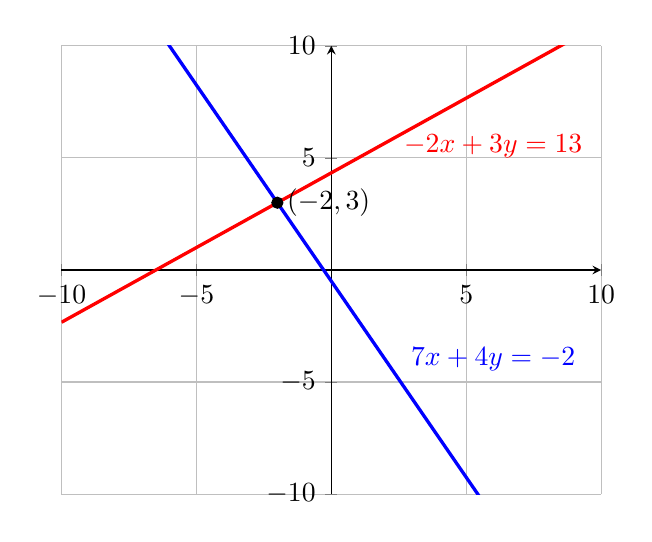
\begin{tikzpicture}
            \begin{axis}[
                axis lines=middle,
                grid=both,
                grid,
                ymin=-10,
                ymax=10,
                xmin=-10, 
                xmax=10
                ]       
                \addplot[mark=none, blue, very thick] coordinates {(-10,17) (10,-18)} node[above] at (axis cs:6,-5) {$7x+4y=-2$};
                \addplot[mark=none, red, very thick] coordinates {(-10,-2.3333) (10,11)} node[below] at (axis cs:6,6.5) {$-2x+3y=13$};
                \addplot[mark=*] coordinates {(-2,3)} node[right] at (axis cs:-2,3) {$(-2,3)$};
            \end{axis}
        \end{tikzpicture}
    \end{center}

    这种可视化方法也适用于三个方程和三个未知数的方程组,但这需要在三维空间中绘制图线。这在实践中可能很难做到,但在技术上是可行的。同样的概念也适用于多个方程和多个未知数,但在四维或更高维上画``线''对我们人类来说是可能是无法想象的!
\end{method}

\begin{method}{多于两个变量:消元!}
    该方法的下一部分建立在第一部分的基础上,通过不断应用第一部分的方法,将两个以上方程(和未知数)的方程组简化为更小的方程组,最终得到两个方程和两个未知数的方程组。我们通过一个三个方程和三个未知数的方程组来说明该方法,如下所示:
    $$
    \begin{cases}
        \enspace\: 6x - 3y + \enspace z = -1 \\
        -3x + 4y - 2z = 12 \\
        \enspace\: 5x + \enspace y + 8z = 6
    \end{cases}
    $$
    第一个目标是消除三个变量中的一个。本质上,这可以通过两种方式之一来完成,就像两个方程和两个未知数的方法一样。假设我们要从方程组中消除 $z$;我们可以尝试以某种方式用 $x$ 和 $y$ 来表示 $z$ 并代入,或者我们可以将某些方程乘以系数并相加,从而消除 $z$。这里唯一的区别是,无论我们选择哪种方法,我们都需要执行两次。我们用第一个方程得到
    \[z = -6x + 3y - 1\]
    将 $z$ 的表达式代入第二个和第三个方程后,我们将得到一个由两个方程和两个未知数组成的方程组。

    思考这个问题的一种方法是,我们需要来自所有三个方程的信息才能最终得出答案,因此在将方程组简化为两个方程时,我们需要以某种方式保留来自所有三个原始方程的信息。$z$ 的表达式来自第一个方程,因此我们需要将其代入其他两个方程以保留我们需要的所有信息。

    将其与以下步骤序列进行比较:整理第一个方程以分离 $z$ 并将其代入第二个方程,然后整理第二个方程式以分离 $z$,将其代入第一个方程。会发生什么?直觉告诉我们,在某种程度上``丢失''了第三个方程的信息,没错,我们将获得一个由两个方程和两个未知数组成的方程组,但它没有足够的信息得到 $x$ 和 $y$ 的唯一解。如果你真的执行了我们刚才描述的步骤(试着这样做来检查我们的工作),化简到最简后,可以得到以下两个方程的``方程组'':
    $$
    \begin{cases}
        9x - 2y = 10 \\
        \frac{9}{2}x - \:y = 5
    \end{cases}
    $$
    这两个方程其实是同一个方程!因此,我们实际上无法求解 $x$ 和 $y$ 的唯一值。

    让我们回到原来的位置,将上面 $z$ 的表达式代入第二和第三个方程
    \begin{align*}
        -3x + 4y - 2 \cdot (-6x + 3y - 1) &= 12 \\
        5x + y + 8 \cdot (-6x + 3y - 1) &= 6
    \end{align*}
    然后化简
    \begin{align*}
        9x - 2y &= 10 \\
        -43x + 25y &= 14
    \end{align*}
    应用第一个问题中的方法之一将解出 $(x, y) = (2, 4)$。有了这两个值,我们就可以代入三个原始方程中的任意一个并求出 $z$;更好的做法是,我们可以使用从第一个方程中得到的 $z$ 的表达式:
    \[z = -6x + 3y - 1 = -6 \cdot (2) + 3 \cdot 4 = 1 = -12 + 12 - 1 = -1\]
\end{method}

\begin{method}{多于两个变量:另一种消元方法!}
    将方程组从三个方程简化为两个方程的另一种方法与前面的``乘加''法有关。使用上面具有三个方程的方程组,我们可能会注意到,第一个方程乘以 $8$,第二个方程乘以 $4$ 后,所有三个方程中 $z$ 的系数都是 $\pm 8$。这使我们能够以简便的方式对方程进行加/减,将方程组简化为两个方程和两个未知数。具体来说,让我们做一遍刚才提到的操作
    \begin{align*}
        48x - 24y + 8z &= -8 \\
        -12x + 16y - 8z &= 48 \\
        5x + y + 8z &= 6
    \end{align*}
    然后将第一个方程与第二个方程相加
    \begin{align*}
        (48x - 12x) + (-24y + 16y) + (8z - 8z) &= -8 + 48 \\
        36x - 8y &= 40
    \end{align*}
    接着将第二个方程与第三个方程相加
    \begin{align*}
        (-12x + 5x) + (16y + y) + (-8z + 8z) &= 48 + 6 \\
        -7x + 17y &= 54
    \end{align*}
    上面操作将产生了两个仅包含 $x$和 $y$ 的方程;此外,我们结合了所有三个原始方程的信息来生成这些方程,所以我们可以确信我们没有``丢失''任何东西。用我们之前讨论的任意一种方法解此新方程组
    $$
    \begin{cases}
        \: 36x - \enspace 8y = 40 \\
        -7x + 17y = 54  
    \end{cases}
    $$
    都会解得 $(x, y) = (2, 4)$。将 $x$ 和 $y$ 的值代入三个原始方程中的任意一个并求出 $z$,即可得到我们要求的最终答案。

    我们也可以执行类似的步骤,从方程组中消除 $y$;例如,我们可以将第一个方程乘以 $4$ 与第二个方程乘以 $3$ 相加,然后用第二个方程减去第三个方程乘以 $4$。这些方法中的任何一种都会得到相同的最终答案,只是其中一些可能会缩短算术步骤或带来``更好计算''的数字(即更少的分数,更小的乘法,等等)。求解具有更多方程的方程组的一般过程:将方程相乘并相加,从方程组中消除一个变量,然后继续这样做,直到只有两个方程和两个未知数;然后,求解这两个变量的值,并反向代入运算,用这些值来求解已消除变量的值。
\end{method}

\subsubsection*{代数练习}

\begin{problem}
    求解关于 $(x, y, z)$ 的以下方程组:

    $$
    \begin{cases}
        \enspace x+y+z=15\\
        2x-y+z=8\\
        x-2y-z=-2
    \end{cases}
    $$

    求解关于 $(x, y, z)$ 的类似方程组:

    $$
    \begin{cases}
        \enspace x+y+z=15\\
        2x-y+z=9\\
        x-2y-z=-2
    \end{cases}
    $$

    比较两个方程组之间 $x$、$y$ 和 $z$ 值的变化。

    哪个变量变化最大?哪个最少?这些变化的比例是多少?

    通过改变方程组第二个方程右侧的常数,你可以使这个比率变多大/多小?
\end{problem}

\begin{problem}
    父亲、母亲和儿子坐在餐厅里吃饭,这时另一个由父亲、母亲和儿子组成的家庭走过来。第二个家庭惊讶于他们与第一个家庭如此相似,于是就问第一个家庭:``你们三个多大了?我猜我们的年龄都差不多''。第一个家庭的父亲恰好是一位数学家,不愿意轻易泄露家人的年龄,于是用一种巧妙的方式``透露''给其他人。他说:``我们现在的年龄加起来是 $72$ 岁,而我恰好是我儿子的六倍。然而,将来当我只是他年龄的两倍时,我们的年龄加起来将是我们现在年龄加起来的两倍。你猜我们多少岁?''\\
    三个家庭成员的年龄有多大?
\end{problem}